% Options for packages loaded elsewhere
\PassOptionsToPackage{unicode}{hyperref}
\PassOptionsToPackage{hyphens}{url}
%
\documentclass[
]{article}
\usepackage{amsmath,amssymb}
\usepackage{iftex}
\ifPDFTeX
  \usepackage[T1]{fontenc}
  \usepackage[utf8]{inputenc}
  \usepackage{textcomp} % provide euro and other symbols
\else % if luatex or xetex
  \usepackage{unicode-math} % this also loads fontspec
  \defaultfontfeatures{Scale=MatchLowercase}
  \defaultfontfeatures[\rmfamily]{Ligatures=TeX,Scale=1}
\fi
\usepackage{lmodern}
\ifPDFTeX\else
  % xetex/luatex font selection
\fi
% Use upquote if available, for straight quotes in verbatim environments
\IfFileExists{upquote.sty}{\usepackage{upquote}}{}
\IfFileExists{microtype.sty}{% use microtype if available
  \usepackage[]{microtype}
  \UseMicrotypeSet[protrusion]{basicmath} % disable protrusion for tt fonts
}{}
\makeatletter
\@ifundefined{KOMAClassName}{% if non-KOMA class
  \IfFileExists{parskip.sty}{%
    \usepackage{parskip}
  }{% else
    \setlength{\parindent}{0pt}
    \setlength{\parskip}{6pt plus 2pt minus 1pt}}
}{% if KOMA class
  \KOMAoptions{parskip=half}}
\makeatother
\usepackage{xcolor}
\usepackage[margin=1in]{geometry}
\usepackage{color}
\usepackage{fancyvrb}
\newcommand{\VerbBar}{|}
\newcommand{\VERB}{\Verb[commandchars=\\\{\}]}
\DefineVerbatimEnvironment{Highlighting}{Verbatim}{commandchars=\\\{\}}
% Add ',fontsize=\small' for more characters per line
\usepackage{framed}
\definecolor{shadecolor}{RGB}{248,248,248}
\newenvironment{Shaded}{\begin{snugshade}}{\end{snugshade}}
\newcommand{\AlertTok}[1]{\textcolor[rgb]{0.94,0.16,0.16}{#1}}
\newcommand{\AnnotationTok}[1]{\textcolor[rgb]{0.56,0.35,0.01}{\textbf{\textit{#1}}}}
\newcommand{\AttributeTok}[1]{\textcolor[rgb]{0.13,0.29,0.53}{#1}}
\newcommand{\BaseNTok}[1]{\textcolor[rgb]{0.00,0.00,0.81}{#1}}
\newcommand{\BuiltInTok}[1]{#1}
\newcommand{\CharTok}[1]{\textcolor[rgb]{0.31,0.60,0.02}{#1}}
\newcommand{\CommentTok}[1]{\textcolor[rgb]{0.56,0.35,0.01}{\textit{#1}}}
\newcommand{\CommentVarTok}[1]{\textcolor[rgb]{0.56,0.35,0.01}{\textbf{\textit{#1}}}}
\newcommand{\ConstantTok}[1]{\textcolor[rgb]{0.56,0.35,0.01}{#1}}
\newcommand{\ControlFlowTok}[1]{\textcolor[rgb]{0.13,0.29,0.53}{\textbf{#1}}}
\newcommand{\DataTypeTok}[1]{\textcolor[rgb]{0.13,0.29,0.53}{#1}}
\newcommand{\DecValTok}[1]{\textcolor[rgb]{0.00,0.00,0.81}{#1}}
\newcommand{\DocumentationTok}[1]{\textcolor[rgb]{0.56,0.35,0.01}{\textbf{\textit{#1}}}}
\newcommand{\ErrorTok}[1]{\textcolor[rgb]{0.64,0.00,0.00}{\textbf{#1}}}
\newcommand{\ExtensionTok}[1]{#1}
\newcommand{\FloatTok}[1]{\textcolor[rgb]{0.00,0.00,0.81}{#1}}
\newcommand{\FunctionTok}[1]{\textcolor[rgb]{0.13,0.29,0.53}{\textbf{#1}}}
\newcommand{\ImportTok}[1]{#1}
\newcommand{\InformationTok}[1]{\textcolor[rgb]{0.56,0.35,0.01}{\textbf{\textit{#1}}}}
\newcommand{\KeywordTok}[1]{\textcolor[rgb]{0.13,0.29,0.53}{\textbf{#1}}}
\newcommand{\NormalTok}[1]{#1}
\newcommand{\OperatorTok}[1]{\textcolor[rgb]{0.81,0.36,0.00}{\textbf{#1}}}
\newcommand{\OtherTok}[1]{\textcolor[rgb]{0.56,0.35,0.01}{#1}}
\newcommand{\PreprocessorTok}[1]{\textcolor[rgb]{0.56,0.35,0.01}{\textit{#1}}}
\newcommand{\RegionMarkerTok}[1]{#1}
\newcommand{\SpecialCharTok}[1]{\textcolor[rgb]{0.81,0.36,0.00}{\textbf{#1}}}
\newcommand{\SpecialStringTok}[1]{\textcolor[rgb]{0.31,0.60,0.02}{#1}}
\newcommand{\StringTok}[1]{\textcolor[rgb]{0.31,0.60,0.02}{#1}}
\newcommand{\VariableTok}[1]{\textcolor[rgb]{0.00,0.00,0.00}{#1}}
\newcommand{\VerbatimStringTok}[1]{\textcolor[rgb]{0.31,0.60,0.02}{#1}}
\newcommand{\WarningTok}[1]{\textcolor[rgb]{0.56,0.35,0.01}{\textbf{\textit{#1}}}}
\usepackage{graphicx}
\makeatletter
\def\maxwidth{\ifdim\Gin@nat@width>\linewidth\linewidth\else\Gin@nat@width\fi}
\def\maxheight{\ifdim\Gin@nat@height>\textheight\textheight\else\Gin@nat@height\fi}
\makeatother
% Scale images if necessary, so that they will not overflow the page
% margins by default, and it is still possible to overwrite the defaults
% using explicit options in \includegraphics[width, height, ...]{}
\setkeys{Gin}{width=\maxwidth,height=\maxheight,keepaspectratio}
% Set default figure placement to htbp
\makeatletter
\def\fps@figure{htbp}
\makeatother
\setlength{\emergencystretch}{3em} % prevent overfull lines
\providecommand{\tightlist}{%
  \setlength{\itemsep}{0pt}\setlength{\parskip}{0pt}}
\setcounter{secnumdepth}{-\maxdimen} % remove section numbering
\ifLuaTeX
  \usepackage{selnolig}  % disable illegal ligatures
\fi
\usepackage{bookmark}
\IfFileExists{xurl.sty}{\usepackage{xurl}}{} % add URL line breaks if available
\urlstyle{same}
\hypersetup{
  pdftitle={Análise Prova Brasil 2011},
  hidelinks,
  pdfcreator={LaTeX via pandoc}}

\title{Análise Prova Brasil 2011}
\author{}
\date{\vspace{-2.5em}}

\begin{document}
\maketitle

Lendo os dados:

\begin{Shaded}
\begin{Highlighting}[]
\FunctionTok{setwd}\NormalTok{(}\StringTok{".."}\NormalTok{) }\CommentTok{\# acessar os dados}
\NormalTok{arquivo }\OtherTok{\textless{}{-}} \StringTok{"dados/Amostra\_g01\_Adrielly\_Amanda\_Erick\_Raquel.xlsx"}
\NormalTok{arquivo\_amostra }\OtherTok{\textless{}{-}} \StringTok{"dados/Amostra\_50\_linhas.xlsx"}

\CommentTok{\# variáveis globais}
\NormalTok{dados }\OtherTok{\textless{}{-}} \FunctionTok{read\_excel}\NormalTok{(arquivo) }\CommentTok{\# caso queria testar para a amostra}
\NormalTok{amostra }\OtherTok{\textless{}{-}} \FunctionTok{read\_excel}\NormalTok{(arquivo\_amostra)}
\NormalTok{n }\OtherTok{\textless{}{-}} \FunctionTok{nrow}\NormalTok{(dados) }\CommentTok{\# caso a amostra seja alterada}
\NormalTok{ic }\OtherTok{\textless{}{-}} \FloatTok{1.96} \CommentTok{\# defini com 95\%}
\end{Highlighting}
\end{Shaded}

\section{1. Descrever as características das escolas e o desempenho de
seus estudantes na Prova de Brasil em
2011.}\label{descrever-as-caracteruxedsticas-das-escolas-e-o-desempenho-de-seus-estudantes-na-prova-de-brasil-em-2011.}

ui \textless- fluidPage( titlePanel(``Dashboard Interativo Prova Brasil
2011''),

sidebarLayout( sidebarPanel( selectInput(``x\_var'', label = ``Escolha a
variável no eixo X'', choices = c(``PARTICIPACAO'', ``TAM\_ESCOLA'',
``MATRICULADOS'',``TAM\_MUN'', ``ADM'', ``LOCAL'', ``REG''), selected =
``PARTICIPACAO''),

\begin{verbatim}
  selectInput("y_var", 
              label = "Escolha a variável no eixo Y",
              choices = c("NOTA_LP", "NOTA_MT"),
              selected = "NOTA_LP"),
  
  selectInput("color_var", 
              label = "Escolha a variável para cor",
              choices = c("REG", "LOCAL", "ADM"),
              selected = "REG")
),

mainPanel(
  plotlyOutput("grafico")
)
\end{verbatim}

) )

server \textless- function(input, output)\{

output\(grafico <- renderPlotly({
    x_var <- input\)x\_var y\_var \textless- input\(y_var
    color_var <- input\)color\_var

\begin{verbatim}
plot_ly(data = dados, 
        x = ~get(x_var), 
        y = ~get(y_var), 
        type = 'scatter', 
        mode = 'markers', 
        color = ~get(color_var), 
        text = ~paste("ID: ", ID, "<br>Local: ", LOCAL),
        marker = list(size = 10)) %>%
  layout(title = paste("Relação entre", x_var, "e", y_var),
         xaxis = list(title = x_var),
         yaxis = list(title = y_var))
\end{verbatim}

\}) \}

shinyApp(ui = ui, server = server)

\section{2. Estimar a proporção de escolas que menos de 75\% de seus
estudantes participaram da Prova Brasil em
2011.}\label{estimar-a-proporuxe7uxe3o-de-escolas-que-menos-de-75-de-seus-estudantes-participaram-da-prova-brasil-em-2011.}

\begin{Shaded}
\begin{Highlighting}[]
\NormalTok{dados}\SpecialCharTok{$}\NormalTok{BAIXA\_PARTICIPACAO }\OtherTok{\textless{}{-}}\NormalTok{ dados}\SpecialCharTok{$}\NormalTok{PARTICIPACAO }\SpecialCharTok{\textless{}} \DecValTok{75}
\NormalTok{proporcao }\OtherTok{\textless{}{-}} \FunctionTok{mean}\NormalTok{(dados}\SpecialCharTok{$}\NormalTok{BAIXA\_PARTICIPACAO)}
\FunctionTok{print}\NormalTok{(proporcao)}
\end{Highlighting}
\end{Shaded}

\begin{verbatim}
## [1] 0.105
\end{verbatim}

\begin{Shaded}
\begin{Highlighting}[]
\NormalTok{erro\_padrao }\OtherTok{\textless{}{-}} \FunctionTok{sqrt}\NormalTok{(proporcao }\SpecialCharTok{*}\NormalTok{ (}\DecValTok{1}\SpecialCharTok{{-}}\NormalTok{proporcao)}\SpecialCharTok{/}\NormalTok{n)}
\NormalTok{ic\_inf }\OtherTok{\textless{}{-}}\NormalTok{ proporcao}\SpecialCharTok{{-}}\NormalTok{ic}\SpecialCharTok{*}\NormalTok{erro\_padrao}
\NormalTok{ic\_sup }\OtherTok{\textless{}{-}}\NormalTok{ proporcao}\SpecialCharTok{+}\NormalTok{ic}\SpecialCharTok{*}\NormalTok{erro\_padrao}

\CommentTok{\# coloquei 95\% mas poderia ser outro}
\FunctionTok{cat}\NormalTok{(}\FunctionTok{sprintf}\NormalTok{(}\StringTok{"IC[\%.4f ± \%.4f]"}\NormalTok{, proporcao, ic }\SpecialCharTok{*}\NormalTok{ erro\_padrao), }\StringTok{"}\SpecialCharTok{\textbackslash{}n}\StringTok{"}\NormalTok{)}
\end{Highlighting}
\end{Shaded}

\begin{verbatim}
## IC[0.1050 ± 0.0425]
\end{verbatim}

\begin{Shaded}
\begin{Highlighting}[]
\FunctionTok{cat}\NormalTok{(}\FunctionTok{sprintf}\NormalTok{(}\StringTok{"IC[\%.4f; \%.4f]"}\NormalTok{, ic\_inf, ic\_sup))}
\end{Highlighting}
\end{Shaded}

\begin{verbatim}
## IC[0.0625; 0.1475]
\end{verbatim}

\begin{Shaded}
\begin{Highlighting}[]
\CommentTok{\# obs: escolher o mais usual}
\end{Highlighting}
\end{Shaded}

\#3. Estimar a proficiência média em Língua Portuguesa e em Matemática
das escolas na Prova Brasil em 2011.

\begin{Shaded}
\begin{Highlighting}[]
\CommentTok{\# Língua portuguesa}
\NormalTok{media\_pt }\OtherTok{\textless{}{-}} \FunctionTok{mean}\NormalTok{(dados}\SpecialCharTok{$}\NormalTok{NOTA\_LP)}
\NormalTok{erro\_pt }\OtherTok{\textless{}{-}} \FunctionTok{sd}\NormalTok{(dados}\SpecialCharTok{$}\NormalTok{NOTA\_LP)}\SpecialCharTok{/}\FunctionTok{sqrt}\NormalTok{(n)}
\NormalTok{ic\_lp\_inf }\OtherTok{\textless{}{-}}\NormalTok{ media\_pt }\SpecialCharTok{{-}}\NormalTok{ ic }\SpecialCharTok{*}\NormalTok{ erro\_pt}
\NormalTok{ic\_lp\_sup }\OtherTok{\textless{}{-}}\NormalTok{ media\_pt }\SpecialCharTok{+}\NormalTok{ ic }\SpecialCharTok{*}\NormalTok{ erro\_pt}

\FunctionTok{cat}\NormalTok{(}\FunctionTok{sprintf}\NormalTok{(}\StringTok{"IC língua portuguesa: [\%.2f ± \%.2f]}\SpecialCharTok{\textbackslash{}n}\StringTok{"}\NormalTok{, media\_pt, ic }\SpecialCharTok{*}\NormalTok{ erro\_pt))}
\end{Highlighting}
\end{Shaded}

\begin{verbatim}
## IC língua portuguesa: [182.77 ± 3.30]
\end{verbatim}

\begin{Shaded}
\begin{Highlighting}[]
\FunctionTok{cat}\NormalTok{(}\FunctionTok{sprintf}\NormalTok{(}\StringTok{"IC língua portuguesa: [\%.2f; \%.2f]}\SpecialCharTok{\textbackslash{}n}\StringTok{"}\NormalTok{, ic\_lp\_inf, ic\_lp\_sup))}
\end{Highlighting}
\end{Shaded}

\begin{verbatim}
## IC língua portuguesa: [179.46; 186.07]
\end{verbatim}

\begin{Shaded}
\begin{Highlighting}[]
\CommentTok{\# Matemática}
\NormalTok{media\_mt }\OtherTok{\textless{}{-}} \FunctionTok{mean}\NormalTok{(dados}\SpecialCharTok{$}\NormalTok{NOTA\_MT)}
\NormalTok{erro\_mt }\OtherTok{\textless{}{-}} \FunctionTok{sd}\NormalTok{(dados}\SpecialCharTok{$}\NormalTok{NOTA\_MT)}\SpecialCharTok{/}\FunctionTok{sqrt}\NormalTok{(n)}
\NormalTok{ic\_mt\_inf }\OtherTok{\textless{}{-}}\NormalTok{ media\_mt }\SpecialCharTok{{-}}\NormalTok{ ic }\SpecialCharTok{*}\NormalTok{ erro\_mt}
\NormalTok{ic\_mt\_sup }\OtherTok{\textless{}{-}}\NormalTok{ media\_mt }\SpecialCharTok{+}\NormalTok{ ic }\SpecialCharTok{*}\NormalTok{ erro\_mt}

\FunctionTok{cat}\NormalTok{(}\FunctionTok{sprintf}\NormalTok{(}\StringTok{"IC matemática: [\%.2f ± \%.2f]}\SpecialCharTok{\textbackslash{}n}\StringTok{"}\NormalTok{, media\_mt, ic }\SpecialCharTok{*}\NormalTok{ erro\_mt))}
\end{Highlighting}
\end{Shaded}

\begin{verbatim}
## IC matemática: [201.36 ± 3.80]
\end{verbatim}

\begin{Shaded}
\begin{Highlighting}[]
\FunctionTok{cat}\NormalTok{(}\FunctionTok{sprintf}\NormalTok{(}\StringTok{"IC matemática: [\%.2f; \%.2f]}\SpecialCharTok{\textbackslash{}n}\StringTok{"}\NormalTok{, ic\_mt\_inf, ic\_mt\_sup))}
\end{Highlighting}
\end{Shaded}

\begin{verbatim}
## IC matemática: [197.56; 205.16]
\end{verbatim}

\section{4: Verificar se houve melhora do resultado da Prova Brasil de
2009 para
2011}\label{verificar-se-houve-melhora-do-resultado-da-prova-brasil-de-2009-para-2011}

\begin{Shaded}
\begin{Highlighting}[]
\FunctionTok{cat}\NormalTok{(}\StringTok{"Nomes das colunas:}\SpecialCharTok{\textbackslash{}n}\StringTok{"}\NormalTok{)}
\end{Highlighting}
\end{Shaded}

\begin{verbatim}
## Nomes das colunas:
\end{verbatim}

\begin{Shaded}
\begin{Highlighting}[]
\FunctionTok{print}\NormalTok{(}\FunctionTok{colnames}\NormalTok{(amostra))}
\end{Highlighting}
\end{Shaded}

\begin{verbatim}
##  [1] "ID"           "ANO"          "REG"          "LOCAL"        "TAM_MUN"     
##  [6] "ADM"          "TAM_ESCOLA"   "MATRICULADOS" "PARTICIPACAO" "NOTA_LP"     
## [11] "NOTA_MT"
\end{verbatim}

\begin{Shaded}
\begin{Highlighting}[]
\CommentTok{\# Verificar se há dados nas colunas de interesse}
\FunctionTok{cat}\NormalTok{(}\StringTok{"}\SpecialCharTok{\textbackslash{}n}\StringTok{Quantidade de valores não{-}NA em Língua Portuguesa (NOTA\_LP):"}\NormalTok{, }\FunctionTok{sum}\NormalTok{(}\SpecialCharTok{!}\FunctionTok{is.na}\NormalTok{(amostra}\SpecialCharTok{$}\NormalTok{NOTA\_LP)), }\StringTok{"}\SpecialCharTok{\textbackslash{}n}\StringTok{"}\NormalTok{)}
\end{Highlighting}
\end{Shaded}

\begin{verbatim}
## 
## Quantidade de valores não-NA em Língua Portuguesa (NOTA_LP): 50
\end{verbatim}

\begin{Shaded}
\begin{Highlighting}[]
\FunctionTok{cat}\NormalTok{(}\StringTok{"Quantidade de valores não{-}NA em Matemática (NOTA\_MT):"}\NormalTok{, }\FunctionTok{sum}\NormalTok{(}\SpecialCharTok{!}\FunctionTok{is.na}\NormalTok{(amostra}\SpecialCharTok{$}\NormalTok{NOTA\_MT)), }\StringTok{"}\SpecialCharTok{\textbackslash{}n}\StringTok{"}\NormalTok{)}
\end{Highlighting}
\end{Shaded}

\begin{verbatim}
## Quantidade de valores não-NA em Matemática (NOTA_MT): 50
\end{verbatim}

\begin{Shaded}
\begin{Highlighting}[]
\CommentTok{\# Verificar a estrutura dos dados}
\FunctionTok{cat}\NormalTok{(}\StringTok{"}\SpecialCharTok{\textbackslash{}n}\StringTok{Estrutura dos dados:}\SpecialCharTok{\textbackslash{}n}\StringTok{"}\NormalTok{)}
\end{Highlighting}
\end{Shaded}

\begin{verbatim}
## 
## Estrutura dos dados:
\end{verbatim}

\begin{Shaded}
\begin{Highlighting}[]
\FunctionTok{str}\NormalTok{(amostra)}
\end{Highlighting}
\end{Shaded}

\begin{verbatim}
## tibble [50 x 11] (S3: tbl_df/tbl/data.frame)
##  $ ID          : num [1:50] 49 65 153 74 146 122 200 128 47 24 ...
##  $ ANO         : num [1:50] 2011 2011 2011 2011 2011 ...
##  $ REG         : chr [1:50] "CO" "NE" "SE" "NE" ...
##  $ LOCAL       : chr [1:50] "1" "2" "1" "1" ...
##  $ TAM_MUN     : num [1:50] 2 2 3 1 3 1 5 1 1 3 ...
##  $ ADM         : chr [1:50] "3" "3" "3" "3" ...
##  $ TAM_ESCOLA  : num [1:50] 1 2 3 2 2 2 3 2 3 4 ...
##  $ MATRICULADOS: num [1:50] 24 48 53 33 27 25 78 47 61 112 ...
##  $ PARTICIPACAO: num [1:50] 95.8 79.2 100 69.7 92.6 ...
##  $ NOTA_LP     : num [1:50] 178 159 224 153 210 ...
##  $ NOTA_MT     : num [1:50] 192 169 252 170 231 ...
\end{verbatim}

\begin{Shaded}
\begin{Highlighting}[]
\ControlFlowTok{if}\NormalTok{ (}\FunctionTok{sum}\NormalTok{(}\SpecialCharTok{!}\FunctionTok{is.na}\NormalTok{(amostra}\SpecialCharTok{$}\NormalTok{NOTA\_LP)) }\SpecialCharTok{\textgreater{}} \DecValTok{0} \SpecialCharTok{\&\&} \FunctionTok{sum}\NormalTok{(}\SpecialCharTok{!}\FunctionTok{is.na}\NormalTok{(amostra}\SpecialCharTok{$}\NormalTok{NOTA\_MT)) }\SpecialCharTok{\textgreater{}} \DecValTok{0}\NormalTok{) \{}
  \CommentTok{\# Calcular as médias das notas em 2011 (ignorando NAs)}
\NormalTok{  media\_lp\_2011 }\OtherTok{\textless{}{-}} \FunctionTok{mean}\NormalTok{(amostra}\SpecialCharTok{$}\NormalTok{NOTA\_LP, }\AttributeTok{na.rm =} \ConstantTok{TRUE}\NormalTok{)}
\NormalTok{  media\_mat\_2011 }\OtherTok{\textless{}{-}} \FunctionTok{mean}\NormalTok{(amostra}\SpecialCharTok{$}\NormalTok{NOTA\_MT, }\AttributeTok{na.rm =} \ConstantTok{TRUE}\NormalTok{)}

  \CommentTok{\# Valores de 2009}
\NormalTok{  media\_lp\_2009 }\OtherTok{\textless{}{-}} \FloatTok{184.3}
\NormalTok{  media\_mat\_2009 }\OtherTok{\textless{}{-}} \FloatTok{204.3}

  \CommentTok{\# Comparando as médias}
\NormalTok{  melhoria\_lp }\OtherTok{\textless{}{-}}\NormalTok{ media\_lp\_2011 }\SpecialCharTok{{-}}\NormalTok{ media\_lp\_2009}
\NormalTok{  melhoria\_mat }\OtherTok{\textless{}{-}}\NormalTok{ media\_mat\_2011 }\SpecialCharTok{{-}}\NormalTok{ media\_mat\_2009}

  \CommentTok{\# Exibindo os resultados}
  \FunctionTok{cat}\NormalTok{(}\StringTok{"}\SpecialCharTok{\textbackslash{}n}\StringTok{Média de Língua Portuguesa em 2011 (amostra de 50 escolas):"}\NormalTok{, media\_lp\_2011, }\StringTok{"}\SpecialCharTok{\textbackslash{}n}\StringTok{"}\NormalTok{)}
  \FunctionTok{cat}\NormalTok{(}\StringTok{"Média de Matemática em 2011 (amostra de 50 escolas):"}\NormalTok{, media\_mat\_2011, }\StringTok{"}\SpecialCharTok{\textbackslash{}n}\StringTok{"}\NormalTok{)}
  \FunctionTok{cat}\NormalTok{(}\StringTok{"Melhoria em Língua Portuguesa de 2009 para 2011:"}\NormalTok{, melhoria\_lp, }\StringTok{"}\SpecialCharTok{\textbackslash{}n}\StringTok{"}\NormalTok{)}
  \FunctionTok{cat}\NormalTok{(}\StringTok{"Melhoria em Matemática de 2009 para 2011:"}\NormalTok{, melhoria\_mat, }\StringTok{"}\SpecialCharTok{\textbackslash{}n}\StringTok{"}\NormalTok{)}

  \CommentTok{\# Intervalo de confiança para a média de Língua Portuguesa}
\NormalTok{  erro\_padrao\_lp }\OtherTok{\textless{}{-}} \FunctionTok{sd}\NormalTok{(amostra}\SpecialCharTok{$}\NormalTok{NOTA\_LP, }\AttributeTok{na.rm =} \ConstantTok{TRUE}\NormalTok{) }\SpecialCharTok{/} \FunctionTok{sqrt}\NormalTok{(}\FunctionTok{nrow}\NormalTok{(amostra))}
\NormalTok{  ic\_inf\_lp }\OtherTok{\textless{}{-}}\NormalTok{ media\_lp\_2011 }\SpecialCharTok{{-}}\NormalTok{ ic }\SpecialCharTok{*}\NormalTok{ erro\_padrao\_lp}
\NormalTok{  ic\_sup\_lp }\OtherTok{\textless{}{-}}\NormalTok{ media\_lp\_2011 }\SpecialCharTok{+}\NormalTok{ ic }\SpecialCharTok{*}\NormalTok{ erro\_padrao\_lp}

  \FunctionTok{cat}\NormalTok{(}\FunctionTok{sprintf}\NormalTok{(}\StringTok{"IC para Língua Portuguesa [\%.4f; \%.4f]"}\NormalTok{, ic\_inf\_lp, ic\_sup\_lp), }\StringTok{"}\SpecialCharTok{\textbackslash{}n}\StringTok{"}\NormalTok{)}

  \CommentTok{\# Intervalo de confiança para a média de Matemática}
\NormalTok{  erro\_padrao\_mat }\OtherTok{\textless{}{-}} \FunctionTok{sd}\NormalTok{(amostra}\SpecialCharTok{$}\NormalTok{NOTA\_MT, }\AttributeTok{na.rm =} \ConstantTok{TRUE}\NormalTok{) }\SpecialCharTok{/} \FunctionTok{sqrt}\NormalTok{(}\FunctionTok{nrow}\NormalTok{(amostra))}
\NormalTok{  ic\_inf\_mat }\OtherTok{\textless{}{-}}\NormalTok{ media\_mat\_2011 }\SpecialCharTok{{-}}\NormalTok{ ic }\SpecialCharTok{*}\NormalTok{ erro\_padrao\_mat}
\NormalTok{  ic\_sup\_mat }\OtherTok{\textless{}{-}}\NormalTok{ media\_mat\_2011 }\SpecialCharTok{+}\NormalTok{ ic }\SpecialCharTok{*}\NormalTok{ erro\_padrao\_mat}

  \FunctionTok{cat}\NormalTok{(}\FunctionTok{sprintf}\NormalTok{(}\StringTok{"IC para Matemática [\%.4f; \%.4f]"}\NormalTok{, ic\_inf\_mat, ic\_sup\_mat), }\StringTok{"}\SpecialCharTok{\textbackslash{}n}\StringTok{"}\NormalTok{)}
\NormalTok{\} }\ControlFlowTok{else}\NormalTok{ \{}
  \FunctionTok{cat}\NormalTok{(}\StringTok{"}\SpecialCharTok{\textbackslash{}n}\StringTok{Erro: As colunas de notas (NOTA\_LP ou NOTA\_MT) estão vazias ou contêm apenas NA.}\SpecialCharTok{\textbackslash{}n}\StringTok{"}\NormalTok{)}
\NormalTok{\}}
\end{Highlighting}
\end{Shaded}

\begin{verbatim}
## 
## Média de Língua Portuguesa em 2011 (amostra de 50 escolas): 185.2754 
## Média de Matemática em 2011 (amostra de 50 escolas): 204.5528 
## Melhoria em Língua Portuguesa de 2009 para 2011: 0.9754 
## Melhoria em Matemática de 2009 para 2011: 0.2528 
## IC para Língua Portuguesa [178.6215; 191.9293] 
## IC para Matemática [197.0116; 212.0940]
\end{verbatim}

\section{5: Verificar se as notas em Língua Portuguesa e Matemática são
normalmente
distribuídas}\label{verificar-se-as-notas-em-luxedngua-portuguesa-e-matemuxe1tica-suxe3o-normalmente-distribuuxeddas}

\begin{Shaded}
\begin{Highlighting}[]
\ControlFlowTok{if}\NormalTok{ (}\FunctionTok{sum}\NormalTok{(}\SpecialCharTok{!}\FunctionTok{is.na}\NormalTok{(amostra}\SpecialCharTok{$}\NormalTok{NOTA\_LP)) }\SpecialCharTok{\textgreater{}} \DecValTok{0} \SpecialCharTok{\&\&} \FunctionTok{sum}\NormalTok{(}\SpecialCharTok{!}\FunctionTok{is.na}\NormalTok{(amostra}\SpecialCharTok{$}\NormalTok{NOTA\_MT)) }\SpecialCharTok{\textgreater{}} \DecValTok{0}\NormalTok{) \{}
  \CommentTok{\# Teste de Shapiro{-}Wilk para normalidade (ignorando NAs)}
\NormalTok{  shapiro\_lp }\OtherTok{\textless{}{-}} \FunctionTok{shapiro.test}\NormalTok{(}\FunctionTok{na.omit}\NormalTok{(amostra}\SpecialCharTok{$}\NormalTok{NOTA\_LP))}
\NormalTok{  shapiro\_mat }\OtherTok{\textless{}{-}} \FunctionTok{shapiro.test}\NormalTok{(}\FunctionTok{na.omit}\NormalTok{(amostra}\SpecialCharTok{$}\NormalTok{NOTA\_MT))}

  \CommentTok{\# Exibindo os resultados dos testes}
  \FunctionTok{cat}\NormalTok{(}\StringTok{"}\SpecialCharTok{\textbackslash{}n}\StringTok{Teste de Shapiro{-}Wilk para Língua Portuguesa (amostra de 50 escolas):}\SpecialCharTok{\textbackslash{}n}\StringTok{"}\NormalTok{)}
  \FunctionTok{print}\NormalTok{(shapiro\_lp)}
  \FunctionTok{cat}\NormalTok{(}\StringTok{"}\SpecialCharTok{\textbackslash{}n}\StringTok{Teste de Shapiro{-}Wilk para Matemática (amostra de 50 escolas):}\SpecialCharTok{\textbackslash{}n}\StringTok{"}\NormalTok{)}
  \FunctionTok{print}\NormalTok{(shapiro\_mat)}

  \CommentTok{\# Q{-}Q plots para verificação visual da normalidade (ignorando NAs)}
  \FunctionTok{par}\NormalTok{(}\AttributeTok{mfrow =} \FunctionTok{c}\NormalTok{(}\DecValTok{1}\NormalTok{, }\DecValTok{2}\NormalTok{))}
  \FunctionTok{qqnorm}\NormalTok{(}\FunctionTok{na.omit}\NormalTok{(amostra}\SpecialCharTok{$}\NormalTok{NOTA\_LP), }\AttributeTok{main =} \StringTok{"Q{-}Q Plot Língua Portuguesa (amostra de 50 escolas)"}\NormalTok{)}
  \FunctionTok{qqline}\NormalTok{(}\FunctionTok{na.omit}\NormalTok{(amostra}\SpecialCharTok{$}\NormalTok{NOTA\_LP))}
  \FunctionTok{qqnorm}\NormalTok{(}\FunctionTok{na.omit}\NormalTok{(amostra}\SpecialCharTok{$}\NormalTok{NOTA\_MT), }\AttributeTok{main =} \StringTok{"Q{-}Q Plot Matemática (amostra de 50 escolas)"}\NormalTok{)}
  \FunctionTok{qqline}\NormalTok{(}\FunctionTok{na.omit}\NormalTok{(amostra}\SpecialCharTok{$}\NormalTok{NOTA\_MT))}
\NormalTok{\} }\ControlFlowTok{else}\NormalTok{ \{}
  \FunctionTok{cat}\NormalTok{(}\StringTok{"}\SpecialCharTok{\textbackslash{}n}\StringTok{Erro: As colunas de notas (NOTA\_LP ou NOTA\_MT) estão vazias ou contêm apenas NA.}\SpecialCharTok{\textbackslash{}n}\StringTok{"}\NormalTok{)}
\NormalTok{\}}
\end{Highlighting}
\end{Shaded}

\begin{verbatim}
## 
## Teste de Shapiro-Wilk para Língua Portuguesa (amostra de 50 escolas):
## 
##  Shapiro-Wilk normality test
## 
## data:  na.omit(amostra$NOTA_LP)
## W = 0.95974, p-value = 0.08666
## 
## 
## Teste de Shapiro-Wilk para Matemática (amostra de 50 escolas):
## 
##  Shapiro-Wilk normality test
## 
## data:  na.omit(amostra$NOTA_MT)
## W = 0.95881, p-value = 0.07927
\end{verbatim}

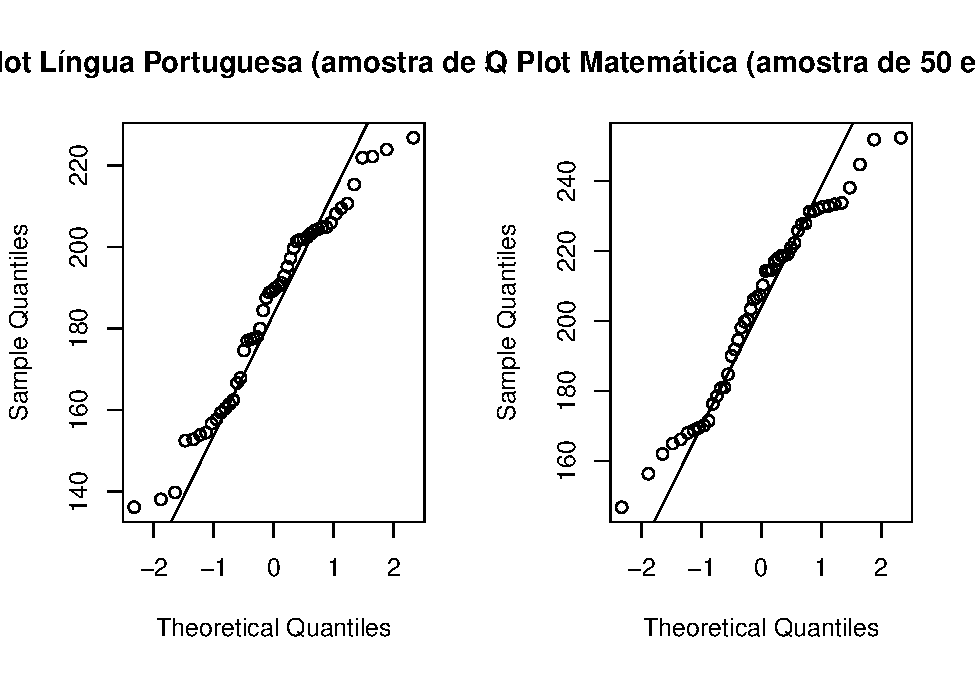
\includegraphics{Analises_files/figure-latex/unnamed-chunk-5-1.pdf}

\section{6: Questão 6}\label{questuxe3o-6}

\section{8. Comparar a proporção de escolas que menos de 75\% de seus
estudantes participaram da Prova Brasil em 2011
segundo:}\label{comparar-a-proporuxe7uxe3o-de-escolas-que-menos-de-75-de-seus-estudantes-participaram-da-prova-brasil-em-2011-segundo}

\subsection{Local da escola}\label{local-da-escola}

\subsubsection{Analise para amostra de
200}\label{analise-para-amostra-de-200}

\begin{Shaded}
\begin{Highlighting}[]
\NormalTok{menor\_75 }\OtherTok{\textless{}{-}}\NormalTok{ dados }\SpecialCharTok{\%\textgreater{}\%}
  \FunctionTok{group\_by}\NormalTok{(LOCAL) }\SpecialCharTok{\%\textgreater{}\%}
  \FunctionTok{summarise}\NormalTok{(}
    \AttributeTok{total =} \FunctionTok{n}\NormalTok{(),}
    \AttributeTok{menor\_que\_75 =} \FunctionTok{sum}\NormalTok{(PARTICIPACAO  }\SpecialCharTok{\textless{}} \DecValTok{75}\NormalTok{),}
    \AttributeTok{prop =} \FunctionTok{round}\NormalTok{(menor\_que\_75 }\SpecialCharTok{/}\NormalTok{ total, }\DecValTok{2}\NormalTok{)}
\NormalTok{  )}

\NormalTok{menor\_75}\SpecialCharTok{$}\NormalTok{LOCAL }\OtherTok{\textless{}{-}}\NormalTok{ menor\_75}\SpecialCharTok{$}\NormalTok{LOCAL }\SpecialCharTok{\%\textgreater{}\%}
  \FunctionTok{factor}\NormalTok{(}\AttributeTok{levels =} \FunctionTok{c}\NormalTok{(}\StringTok{"1"}\NormalTok{, }\StringTok{"2"}\NormalTok{), }\AttributeTok{labels =} \FunctionTok{c}\NormalTok{(}\StringTok{"Urbano"}\NormalTok{, }\StringTok{"Rural"}\NormalTok{))}


\NormalTok{menor\_75 }\SpecialCharTok{\%\textgreater{}\%} 
  \FunctionTok{ggplot}\NormalTok{(}\FunctionTok{aes}\NormalTok{(}\AttributeTok{x =} \FunctionTok{reorder}\NormalTok{(LOCAL, }\SpecialCharTok{{-}}\NormalTok{prop), }\AttributeTok{y =}\NormalTok{ prop, }\AttributeTok{fill =}\NormalTok{ LOCAL)) }\SpecialCharTok{+}
  \FunctionTok{geom\_bar}\NormalTok{(}\AttributeTok{stat =} \StringTok{"identity"}\NormalTok{) }\SpecialCharTok{+}
  \FunctionTok{labs}\NormalTok{(}\AttributeTok{title =} \StringTok{"Proporção de escolas com menos de 75\% de participação por região"}\NormalTok{,}
       \AttributeTok{x =} \StringTok{"Região"}\NormalTok{, }\AttributeTok{y =} \StringTok{"Proporção"}\NormalTok{) }\SpecialCharTok{+}
  \FunctionTok{theme\_bw}\NormalTok{()}
\end{Highlighting}
\end{Shaded}

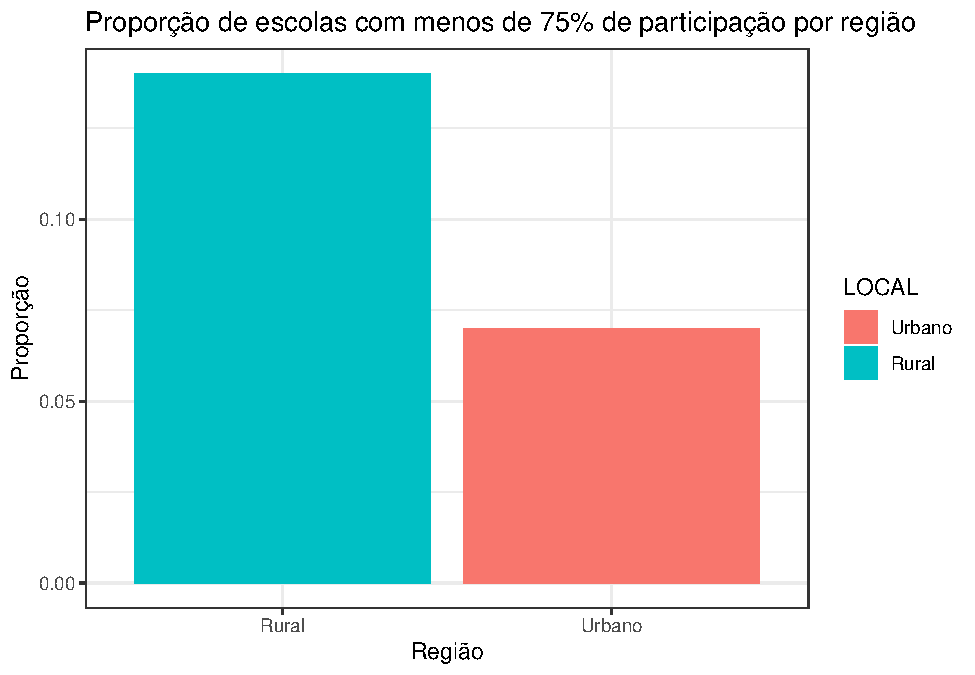
\includegraphics{Analises_files/figure-latex/unnamed-chunk-6-1.pdf}

\subsubsection{Analise para amostra de
50}\label{analise-para-amostra-de-50}

\begin{Shaded}
\begin{Highlighting}[]
\NormalTok{menor\_75 }\OtherTok{\textless{}{-}}\NormalTok{ amostra }\SpecialCharTok{\%\textgreater{}\%}
  \FunctionTok{group\_by}\NormalTok{(LOCAL) }\SpecialCharTok{\%\textgreater{}\%}
  \FunctionTok{summarise}\NormalTok{(}
    \AttributeTok{total =} \FunctionTok{n}\NormalTok{(),}
    \AttributeTok{menor\_que\_75 =} \FunctionTok{sum}\NormalTok{(PARTICIPACAO  }\SpecialCharTok{\textless{}} \DecValTok{75}\NormalTok{),}
    \AttributeTok{prop =} \FunctionTok{round}\NormalTok{(menor\_que\_75 }\SpecialCharTok{/}\NormalTok{ total, }\DecValTok{2}\NormalTok{)}
\NormalTok{  )}

\NormalTok{menor\_75}\SpecialCharTok{$}\NormalTok{LOCAL }\OtherTok{\textless{}{-}}\NormalTok{ menor\_75}\SpecialCharTok{$}\NormalTok{LOCAL }\SpecialCharTok{\%\textgreater{}\%}
  \FunctionTok{factor}\NormalTok{(}\AttributeTok{levels =} \FunctionTok{c}\NormalTok{(}\StringTok{"1"}\NormalTok{, }\StringTok{"2"}\NormalTok{), }\AttributeTok{labels =} \FunctionTok{c}\NormalTok{(}\StringTok{"Urbano"}\NormalTok{, }\StringTok{"Rural"}\NormalTok{))}


\NormalTok{menor\_75 }\SpecialCharTok{\%\textgreater{}\%} 
  \FunctionTok{ggplot}\NormalTok{(}\FunctionTok{aes}\NormalTok{(}\AttributeTok{x =} \FunctionTok{reorder}\NormalTok{(LOCAL, }\SpecialCharTok{{-}}\NormalTok{prop), }\AttributeTok{y =}\NormalTok{ prop, }\AttributeTok{fill =}\NormalTok{ LOCAL)) }\SpecialCharTok{+}
  \FunctionTok{geom\_bar}\NormalTok{(}\AttributeTok{stat =} \StringTok{"identity"}\NormalTok{) }\SpecialCharTok{+}
  \FunctionTok{labs}\NormalTok{(}\AttributeTok{title =} \StringTok{"Proporção de escolas com menos de 75\% de participação por região"}\NormalTok{,}
       \AttributeTok{x =} \StringTok{"Região"}\NormalTok{, }\AttributeTok{y =} \StringTok{"Proporção"}\NormalTok{) }\SpecialCharTok{+}
  \FunctionTok{theme\_bw}\NormalTok{()}
\end{Highlighting}
\end{Shaded}

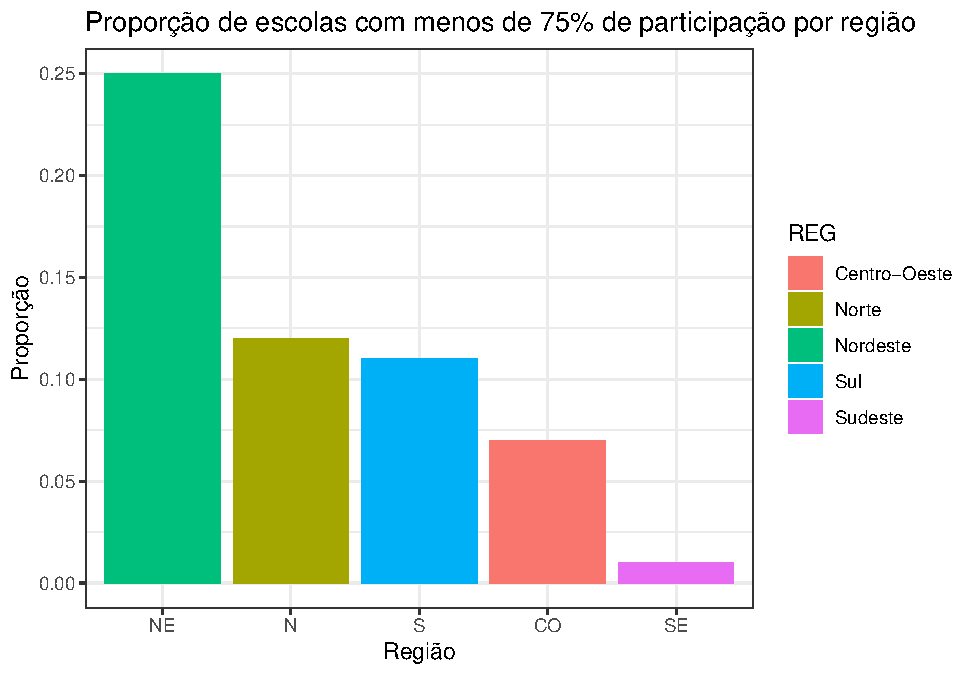
\includegraphics{Analises_files/figure-latex/unnamed-chunk-7-1.pdf}

\subsection{Região de localização da
escola}\label{regiuxe3o-de-localizauxe7uxe3o-da-escola}

\subsubsection{Analise para amostra de
200}\label{analise-para-amostra-de-200-1}

\begin{Shaded}
\begin{Highlighting}[]
\NormalTok{menor\_75 }\OtherTok{\textless{}{-}}\NormalTok{ dados }\SpecialCharTok{\%\textgreater{}\%}
  \FunctionTok{group\_by}\NormalTok{(REG) }\SpecialCharTok{\%\textgreater{}\%}
  \FunctionTok{summarise}\NormalTok{(}
    \AttributeTok{total =} \FunctionTok{n}\NormalTok{(),}
    \AttributeTok{menor\_que\_75 =} \FunctionTok{sum}\NormalTok{(PARTICIPACAO  }\SpecialCharTok{\textless{}} \DecValTok{75}\NormalTok{),}
    \AttributeTok{prop =} \FunctionTok{round}\NormalTok{(menor\_que\_75 }\SpecialCharTok{/}\NormalTok{ total, }\DecValTok{2}\NormalTok{)}
\NormalTok{  )}


\NormalTok{menor\_75 }\SpecialCharTok{\%\textgreater{}\%} 
  \FunctionTok{ggplot}\NormalTok{(}\FunctionTok{aes}\NormalTok{(}\AttributeTok{x =} \FunctionTok{reorder}\NormalTok{(REG, }\SpecialCharTok{{-}}\NormalTok{prop), }\AttributeTok{y =}\NormalTok{ prop, }\AttributeTok{fill =}\NormalTok{ REG)) }\SpecialCharTok{+}
  \FunctionTok{geom\_bar}\NormalTok{(}\AttributeTok{stat =} \StringTok{"identity"}\NormalTok{) }\SpecialCharTok{+}
  \FunctionTok{labs}\NormalTok{(}\AttributeTok{title =} \StringTok{"Proporção de escolas com menos de 75\% de participação por região"}\NormalTok{,}
       \AttributeTok{x =} \StringTok{"Região"}\NormalTok{, }\AttributeTok{y =} \StringTok{"Proporção"}\NormalTok{) }\SpecialCharTok{+}
  \FunctionTok{scale\_fill\_discrete}\NormalTok{(}
    \AttributeTok{labels =} \FunctionTok{c}\NormalTok{(}\StringTok{"N"} \OtherTok{=} \StringTok{"Norte"}\NormalTok{, }\StringTok{"S"} \OtherTok{=} \StringTok{"Sul"}\NormalTok{, }\StringTok{"CO"} \OtherTok{=} \StringTok{"Centro{-}Oeste"}\NormalTok{, }\StringTok{"NE"} \OtherTok{=} \StringTok{"Nordeste"}\NormalTok{, }\StringTok{"SE"} \OtherTok{=} \StringTok{"Sudeste"}\NormalTok{)}
\NormalTok{  ) }\SpecialCharTok{+}
  \FunctionTok{theme\_bw}\NormalTok{()}
\end{Highlighting}
\end{Shaded}

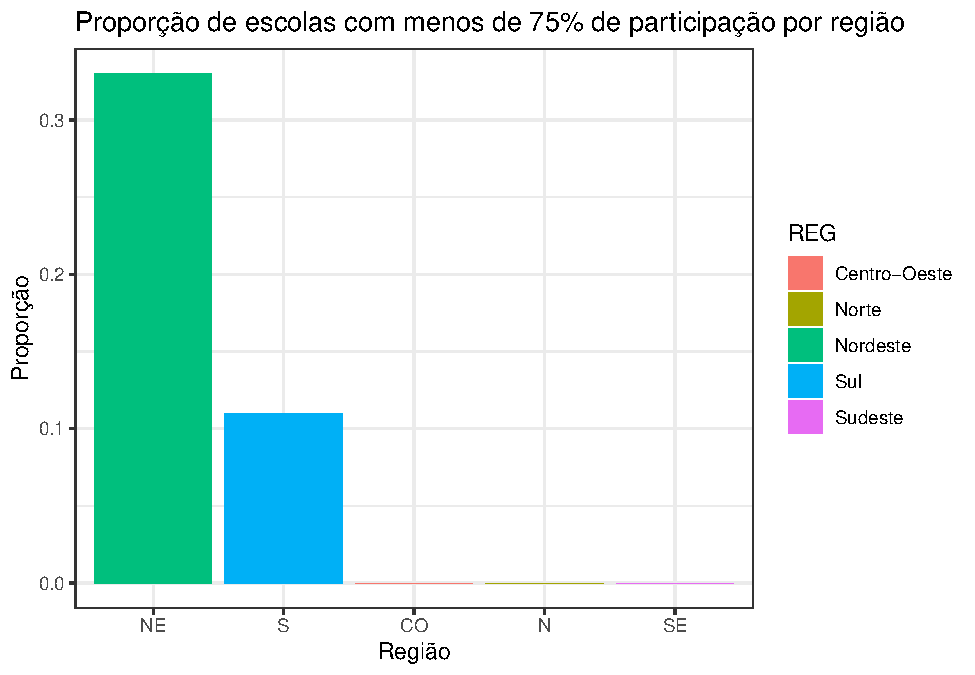
\includegraphics{Analises_files/figure-latex/unnamed-chunk-8-1.pdf}

\subsubsection{Analise para amostra de
50}\label{analise-para-amostra-de-50-1}

\begin{Shaded}
\begin{Highlighting}[]
\NormalTok{menor\_75 }\OtherTok{\textless{}{-}}\NormalTok{ amostra }\SpecialCharTok{\%\textgreater{}\%}
  \FunctionTok{group\_by}\NormalTok{(REG) }\SpecialCharTok{\%\textgreater{}\%}
  \FunctionTok{summarise}\NormalTok{(}
    \AttributeTok{total =} \FunctionTok{n}\NormalTok{(),}
    \AttributeTok{menor\_que\_75 =} \FunctionTok{sum}\NormalTok{(PARTICIPACAO  }\SpecialCharTok{\textless{}} \DecValTok{75}\NormalTok{),}
    \AttributeTok{prop =} \FunctionTok{round}\NormalTok{(menor\_que\_75 }\SpecialCharTok{/}\NormalTok{ total, }\DecValTok{2}\NormalTok{)}
\NormalTok{  )}


\NormalTok{menor\_75 }\SpecialCharTok{\%\textgreater{}\%} 
  \FunctionTok{ggplot}\NormalTok{(}\FunctionTok{aes}\NormalTok{(}\AttributeTok{x =} \FunctionTok{reorder}\NormalTok{(REG, }\SpecialCharTok{{-}}\NormalTok{prop), }\AttributeTok{y =}\NormalTok{ prop, }\AttributeTok{fill =}\NormalTok{ REG)) }\SpecialCharTok{+}
  \FunctionTok{geom\_bar}\NormalTok{(}\AttributeTok{stat =} \StringTok{"identity"}\NormalTok{) }\SpecialCharTok{+}
  \FunctionTok{labs}\NormalTok{(}\AttributeTok{title =} \StringTok{"Proporção de escolas com menos de 75\% de participação por região"}\NormalTok{,}
       \AttributeTok{x =} \StringTok{"Região"}\NormalTok{, }\AttributeTok{y =} \StringTok{"Proporção"}\NormalTok{) }\SpecialCharTok{+}
  \FunctionTok{scale\_fill\_discrete}\NormalTok{(}
    \AttributeTok{labels =} \FunctionTok{c}\NormalTok{(}\StringTok{"N"} \OtherTok{=} \StringTok{"Norte"}\NormalTok{, }\StringTok{"S"} \OtherTok{=} \StringTok{"Sul"}\NormalTok{, }\StringTok{"CO"} \OtherTok{=} \StringTok{"Centro{-}Oeste"}\NormalTok{, }\StringTok{"NE"} \OtherTok{=} \StringTok{"Nordeste"}\NormalTok{, }\StringTok{"SE"} \OtherTok{=} \StringTok{"Sudeste"}\NormalTok{)}
\NormalTok{  ) }\SpecialCharTok{+}
  \FunctionTok{theme\_bw}\NormalTok{()}
\end{Highlighting}
\end{Shaded}

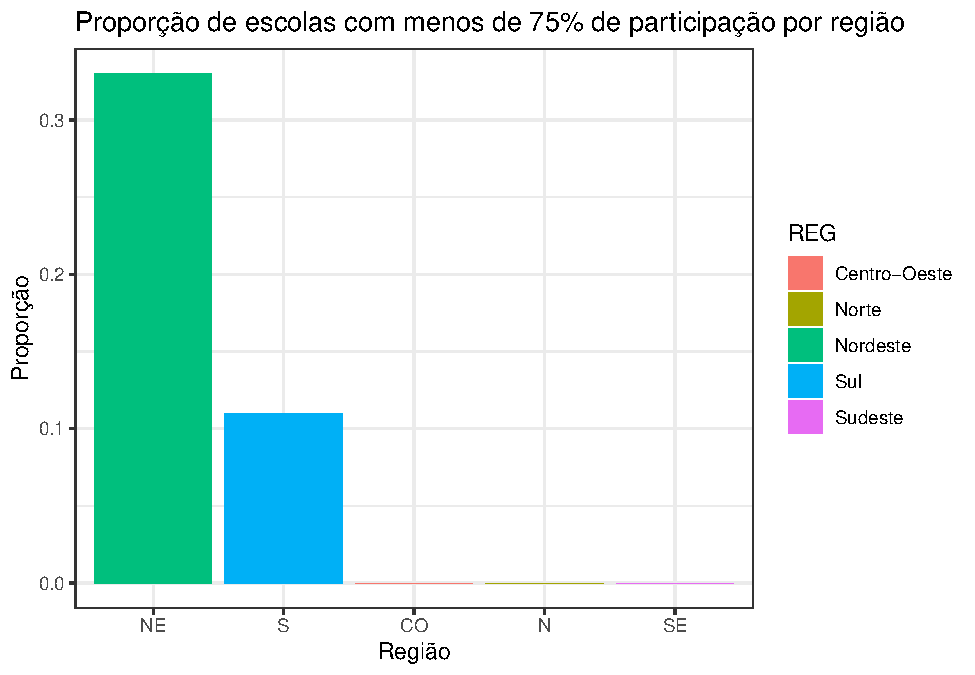
\includegraphics{Analises_files/figure-latex/unnamed-chunk-9-1.pdf}

\section{9. Verificar se:}\label{verificar-se}

\subsection{a. Região e categoria administrativa estão
associadas;}\label{a.-regiuxe3o-e-categoria-administrativa-estuxe3o-associadas}

\subsubsection{Analise para amostra de
200}\label{analise-para-amostra-de-200-2}

\begin{Shaded}
\begin{Highlighting}[]
\CommentTok{\# Teste Qui{-}quadrado }
\FunctionTok{chisq.test}\NormalTok{(dados}\SpecialCharTok{$}\NormalTok{REG,dados}\SpecialCharTok{$}\NormalTok{ADM)}
\end{Highlighting}
\end{Shaded}

\begin{verbatim}
## 
##  Pearson's Chi-squared test
## 
## data:  dados$REG and dados$ADM
## X-squared = 9.2616, df = 4, p-value = 0.05488
\end{verbatim}

\subsubsection{Analise para amostra de
50}\label{analise-para-amostra-de-50-2}

\begin{Shaded}
\begin{Highlighting}[]
\CommentTok{\# Teste Qui{-}quadrado }
\FunctionTok{chisq.test}\NormalTok{(amostra}\SpecialCharTok{$}\NormalTok{REG, amostra}\SpecialCharTok{$}\NormalTok{ADM)}
\end{Highlighting}
\end{Shaded}

\begin{verbatim}
## 
##  Pearson's Chi-squared test
## 
## data:  amostra$REG and amostra$ADM
## X-squared = 10.848, df = 4, p-value = 0.02832
\end{verbatim}

\subsection{b. Tamanho da escola e tamanho do município estão
associados.}\label{b.-tamanho-da-escola-e-tamanho-do-municuxedpio-estuxe3o-associados.}

\subsubsection{Analise para amostra de
200}\label{analise-para-amostra-de-200-3}

\begin{Shaded}
\begin{Highlighting}[]
\FunctionTok{cor.test}\NormalTok{(dados}\SpecialCharTok{$}\NormalTok{TAM\_ESCOLA, dados}\SpecialCharTok{$}\NormalTok{TAM\_MUN, }\AttributeTok{alternative=}\StringTok{"two.sided"}\NormalTok{, }\AttributeTok{method=}\StringTok{"pearson"}\NormalTok{, }\AttributeTok{conf.level=}\DecValTok{0}\NormalTok{,}\DecValTok{95}\NormalTok{)}
\end{Highlighting}
\end{Shaded}

\begin{verbatim}
## 
##  Pearson's product-moment correlation
## 
## data:  dados$TAM_ESCOLA and dados$TAM_MUN
## t = 6.2587, df = 198, p-value = 2.358e-09
## alternative hypothesis: true correlation is not equal to 0
## 0 percent confidence interval:
##  0.4063976 0.4063976
## sample estimates:
##       cor 
## 0.4063976
\end{verbatim}

\subsubsection{Analise para amostra de
50}\label{analise-para-amostra-de-50-3}

\begin{Shaded}
\begin{Highlighting}[]
\FunctionTok{cor.test}\NormalTok{(amostra}\SpecialCharTok{$}\NormalTok{TAM\_ESCOLA, amostra}\SpecialCharTok{$}\NormalTok{TAM\_MUN, }\AttributeTok{alternative=}\StringTok{"two.sided"}\NormalTok{, }\AttributeTok{method=}\StringTok{"pearson"}\NormalTok{, }\AttributeTok{conf.level=}\DecValTok{0}\NormalTok{,}\DecValTok{95}\NormalTok{)}
\end{Highlighting}
\end{Shaded}

\begin{verbatim}
## 
##  Pearson's product-moment correlation
## 
## data:  amostra$TAM_ESCOLA and amostra$TAM_MUN
## t = 2.7022, df = 48, p-value = 0.009493
## alternative hypothesis: true correlation is not equal to 0
## 0 percent confidence interval:
##  0.3633717 0.3633717
## sample estimates:
##       cor 
## 0.3633717
\end{verbatim}

\section{10. Verificar se a nota em Língua Portuguesa é um bom indicador
para predizer a nota existe em Matemática, ou seja se estão
associadas.}\label{verificar-se-a-nota-em-luxedngua-portuguesa-uxe9-um-bom-indicador-para-predizer-a-nota-existe-em-matemuxe1tica-ou-seja-se-estuxe3o-associadas.}

\subsection{Analise para amostra de
200}\label{analise-para-amostra-de-200-4}

\begin{Shaded}
\begin{Highlighting}[]
\FunctionTok{cor.test}\NormalTok{(dados}\SpecialCharTok{$}\NormalTok{NOTA\_LP, dados}\SpecialCharTok{$}\NormalTok{NOTA\_MT, }\AttributeTok{alternative=}\StringTok{"two.sided"}\NormalTok{, }\AttributeTok{method=}\StringTok{"pearson"}\NormalTok{, }\AttributeTok{conf.level=}\DecValTok{0}\NormalTok{,}\DecValTok{95}\NormalTok{)}
\end{Highlighting}
\end{Shaded}

\begin{verbatim}
## 
##  Pearson's product-moment correlation
## 
## data:  dados$NOTA_LP and dados$NOTA_MT
## t = 44.367, df = 198, p-value < 2.2e-16
## alternative hypothesis: true correlation is not equal to 0
## 0 percent confidence interval:
##  0.953207 0.953207
## sample estimates:
##      cor 
## 0.953207
\end{verbatim}

\subsection{Analise para amostra de
50}\label{analise-para-amostra-de-50-4}

\begin{Shaded}
\begin{Highlighting}[]
\FunctionTok{cor.test}\NormalTok{(amostra}\SpecialCharTok{$}\NormalTok{NOTA\_LP, amostra}\SpecialCharTok{$}\NormalTok{NOTA\_MT, }\AttributeTok{alternative=}\StringTok{"two.sided"}\NormalTok{, }\AttributeTok{method=}\StringTok{"pearson"}\NormalTok{, }\AttributeTok{conf.level=}\DecValTok{0}\NormalTok{,}\DecValTok{95}\NormalTok{)}
\end{Highlighting}
\end{Shaded}

\begin{verbatim}
## 
##  Pearson's product-moment correlation
## 
## data:  amostra$NOTA_LP and amostra$NOTA_MT
## t = 22.724, df = 48, p-value < 2.2e-16
## alternative hypothesis: true correlation is not equal to 0
## 0 percent confidence interval:
##  0.9565297 0.9565297
## sample estimates:
##       cor 
## 0.9565297
\end{verbatim}

\end{document}
